%%%%%%%%%%%%%%%%%%%%%%%%
%%%%%%%%% Préambule %%%%%%%%%
%%%%%%%%%%%%%%%%%%%%%%%%
\documentclass[a4paper,12pt]{article}
\usepackage{etex}

%%%%%Langue%%%%%

%%\usepackage[utf8]{inputenc}

\usepackage[T1]{fontenc}
\usepackage{babel} 
%%%%Police%%%%

 %% MATHS BELLES : \usepackage{mathpazo}
 %% TIMES NEW ROMAN :
\usepackage{stmaryrd}
\usepackage{newtxtext, newtxmath}
%%%%%Packages%%%%%

\usepackage[dvipsnames]{xcolor}

\usepackage{afterpage,amsfonts,amsmath,amssymb,amsthm,array,cancel,caption,comment,diagbox,dsfont,enumitem,fancybox,fancyhdr,float, framed,graphics,graphicx,hhline,import,latexsym,lscape,mathabx,multicol,multirow,pdfpages, setspace,subcaption,systeme,tikz,url,xcolor,mdframed}

\usepackage[left=2.5cm, right=2.5cm, top=2.5cm, bottom=2.5cm]{geometry}
\onehalfspacing
\usepackage[french,boxruled]{algorithm2e}
\usepackage[colorlinks=true]{hyperref} 
\usepackage[all]{xy}
\usepackage{dashundergaps}
\usepackage{pgfplots}
\usepackage{pdfpages}
\pgfplotsset{compat=1.18, width=10cm}
\dashundergapssetup{gap-extend-minimum=20pt,gap-extend-percent=20, gap-numbers=false,gap-format=dot,gap-widen=true,teacher-gap-format=dot}

\setlength{\columnsep}{0cm}

\usetikzlibrary{shapes.misc}
\newcommand{\mytimes}{ \tikz[baseline=-.55ex] \node [inner sep=0pt,cross out,draw,line width=1.5pt,minimum size=0.75ex] (a) {};}

\usepackage{tcolorbox}
\tcbuselibrary{theorems}

%%%%Couleurs%%%%

%Version en ligne

\definecolor{t2_red}{RGB}{210,12,70}
\definecolor{t2_blue}{RGB}{12,128,210}
\definecolor{t2_gold}{RGB}{210,180,12}
\definecolor{wooclap_blue}{RGB}{108,151,243}
\definecolor{t2}{RGB}{144,93,146}

%Version Imprimable

%\definecolor{t2_red}{RGB}{0,0,0}
%\definecolor{t2_blue}{RGB}{0,0,0}
%\definecolor{t2_gold}{RGB}{0,0,0}
%\definecolor{wooclap_blue}{RGB}{0,0,0}
%\definecolor{t2}{RGB}{0,0,0}

\hypersetup{urlcolor=t2_red,linkcolor=t2_red,citecolor=t2_red,colorlinks=true}


%%%%%Environnements%%%%%

\newtcbtheorem[number within=section]{defi}{Définition\,}{colback=t2_red!0,colframe=t2_blue,fonttitle=\bfseries}{df}

\newtcbtheorem[number within=section]{prop}{Proposition\,}{colback=t2_red!0,colframe=t2_red,fonttitle=\bfseries}{prop}

\newtcbtheorem[number within=section]{cor}{Corollaire\,}{colback=t2_red!0,colframe=t2_red,fonttitle=\bfseries}{cr}

\newtcbtheorem[number within=section]{theo}{Théorème\,}{colback=t2_red!0,colframe=t2_gold,fonttitle=\bfseries}{th}

\theoremstyle{definition}
%\newtheorem{conv}{Convention}
\newtheorem*{defin}{Définition}
\newtheorem*{ex}{Exemple}
\newtheorem*{exo}{Exercice}
\newtheorem*{corr}{Correction}
\newtheorem*{rap}{Rappel}
\newtheorem*{rem}{Remarque}
\newtheorem*{que}{Question}
\newtheorem*{rems}{Remarques}
\theoremstyle{plain}
\newtheorem*{conj}{Conjecture}
\newtheorem*{demo}{Démonstration}
%\newtheorem{cor}{Corollaire}
%\newtheorem{princ}{Principe}
\newtheorem*{lem}{Lemme}
%\newtheorem{prop}{Proposition}
%\newtheorem{theo}{Théorème}
%\newtheorem*{theo_non_numero}{Théorème}

%\declaretheorem[name=Proposition,sibling=prop]{proprep}

%%%%%Macros%%%%%

%%Ensembles%classiques%%

\def\N{\mathbb{N}}%entiers naturels
\def\Z{\mathbb{Z}}%entiers relatifs
\def\Q{\mathbb{Q}}%rationnels
\def\R{\mathbb{R}}%réels
\def\C{\mathbb{C}}%complexes

%%Algèbre%linéaire%%

\def\codim{\mathrm{codim}}%codimension
\def\ker{\mathrm{ker}\,}%noyau
\def\coker{\mathrm{coker}\,}%conoyau
\def\im{\mathrm{im}\,}%image
\def\id{\mathrm{id}}%application identité
\newcommand\scal[2]{\langle #1,#2\rangle}%produit scalaire

%%Géométrie%différentielle%%

\def\grad{\mathrm{grad}}%gradient
\def\ind{\mathrm{ind}\,}%indice
\def\modu{\mathcal{M}}%espace de modules
\def\moduc{\overline{\mathcal{M}}}%espace de modules compactifié
\def\moducbullet{\overline{\mathcal{M}_\bullet}}%espace de modules avec un point marqué compactifié
\def\ev{\mathrm{ev}}%applications évaluations dans la base
\def\Ev{\mathrm{Ev}}%applications évaluations dans l'espace total
\def\lacet{\ell}%lacet de Morse
\def\lacets{\mathcal{L}}%lacets de Morse
\newcommand\ro{roulement}%roulement-crocodile
\newcommand\Star{{S_\star}}%ensemble du point étoilé et des augmentations
\newcommand\fibrEv{\underset{\Ev}{\boxtimes}}%produit fibré des évaluations dans l'espace total
\newcommand\fibrev{\underset{\mathrm{ev}}{\boxtimes}}%produit fibré des évaluations dans la base
\newcommand\moducmix[1]{\overline{\modu^{#1}}}%espace de modules mixtes
\newcommand\moducmixbul[1]{\overline{\modu^{#1}_\bullet}}%espace de modules à rebonds
\newcommand\moducprime{\overline{\mathcal{M}'}}%espace de modules pour un second jeu de données
\newcommand\rg{\mathfrak{r}}
\newcommand\qg{\mathfrak{q}}
\newcommand\Loop{\mathcal{L}}
\newcommand\push{\Phi}
\newcommand\drum{drumroll}

%%%%%Commandes%%%%%

\def\;{\,\,;\,\,}%point virgule espacé

\def\tq{\,\,\mathrm{t.q.}\,\,}%tel que

\def\iff{\Longleftrightarrow}%équivaut à, la commande initiale ne marche pas

\def\implies{\Longrightarrow}%implique, la commande initiale ne marche pas

\newcommand\fonction[5]{#1:
	\begin{array}{ccc}
		#2&\longrightarrow &#3\\
		#4&\longmapsto &#5
\end{array}}%fonction avec ensembles de départ, d'arrivée et transformation

\newcommand\fonctionbira[5]{#1:
	\begin{array}{ccc}
		#2&\dashrightarrow &#3\\
		#4&\longmapsto &#5
\end{array}}

\newcommand\fonctionnonnommee[4]{\begin{array}{ccc}
		#1 &\longrightarrow& #2\\
		#3 &\longmapsto & #4
\end{array}}%fonction avec ensembles de départ, d'arrivée et transformation, sans nom



%%%%%Bibliographie%%%%%

\bibliographystyle{alpha-en}

%%%%%Style%%%%%

\pagestyle{empty}
\pagestyle{fancy}

\setlength{\headheight}{16pt}
\usepackage{listings}

\definecolor{darkWhite}{rgb}{0.94,0.94,0.94}

\lstset{
	aboveskip=3mm,
	belowskip=-2mm,
	backgroundcolor=\color{darkWhite},
	basicstyle=\footnotesize,
	breakatwhitespace=false,
	breaklines=true,
	captionpos=b,
	commentstyle=\color{red},
	deletekeywords={...},
	escapeinside={\%*}{*)},
	extendedchars=true,
	framexleftmargin=16pt,
	framextopmargin=3pt,
	framexbottommargin=6pt,
	frame=tb,
	keepspaces=true,
	keywordstyle=\color{blue},
	language=C,
	literate=
	{²}{{\textsuperscript{2}}}1
	{⁴}{{\textsuperscript{4}}}1
	{⁶}{{\textsuperscript{6}}}1
	{⁸}{{\textsuperscript{8}}}1
	{€}{{\euro{}}}1
	{é}{{\'e}}1
	{è}{{\`{e}}}1
	{ê}{{\^{e}}}1
	{ë}{{\¨{e}}}1
	{É}{{\'{E}}}1
	{Ê}{{\^{E}}}1
	{û}{{\^{u}}}1
	{ù}{{\`{u}}}1
	{â}{{\^{a}}}1
	{à}{{\`{a}}}1
	{á}{{\'{a}}}1
	{ã}{{\~{a}}}1
	{Á}{{\'{A}}}1
	{Â}{{\^{A}}}1
	{Ã}{{\~{A}}}1
	{ç}{{\c{c}}}1
	{Ç}{{\c{C}}}1
	{õ}{{\~{o}}}1
	{ó}{{\'{o}}}1
	{ô}{{\^{o}}}1
	{Õ}{{\~{O}}}1
	{Ó}{{\'{O}}}1
	{Ô}{{\^{O}}}1
	{î}{{\^{i}}}1
	{Î}{{\^{I}}}1
	{í}{{\'{i}}}1
	{Í}{{\~{Í}}}1,
	morekeywords={*,...},
	numbers=left,
	numbersep=10pt,
	numberstyle=\tiny\color{black},
	rulecolor=\color{black},
	showspaces=false,
	showstringspaces=false,
	showtabs=false,
	stepnumber=1,
	stringstyle=\color{gray},
	tabsize=4,
	title=\lstname,
}

\usepackage[pages=some]{background}

\backgroundsetup{
	scale=1,
	color=black,
	opacity=1,
	angle=0,
	contents={%
		\includegraphics[width=\paperwidth,height=\paperheight]{"figures/PDG_V0"}
	}% %Userpackage for background
}

%%%%%En-tête%%%%%
\date{June 7, 2024.}
\begin{document}

\BgThispage
\begin{titlepage}
	\centering
	\vspace*{3cm}
	{\large LAAS-CNRS.\\
		April 29th - June 14th, 2024.
		\par}
	\rule{0.6\textwidth}{2pt}\\
	{\huge\bfseries Internship report : \\ Evaluation of Spectral Clustering methods. \\\par}
	\rule{0.6\textwidth}{2pt}\\
	\vspace{2cm}
	{\large
		HACINI Malik
		\par }
	\vspace{1cm}
	{\Large\bfseries Supervised by\par} \:
	{\large JONCKHEERE Matthieu\par}
	
\end{titlepage}

\begin{abstract}
	Placeholder
\end{abstract}
\tableofcontents
\section{Introduction}
Clustering data is crucial in various fields as it allows us to identify patterns, group similar entities together and derive meaningful insights from large datasets. In virtually every
scientific field dealing with empirical data, people attempt to get a first impression on their data by
trying to identify groups of “similar behavior” in their data. These fields include machine learning where it is referred to as unsupervised learning, healthcare where clustering techniques are used to identify groups of patients with similar medical characteristics facilitating the conducting of studies and marketing where clustering allows businesses to segment customers based on arbitrary chosen criteria, often used to personalize advertisement. To perform clustering, algorithms are built using mathematical tools from probability theory, statistics, linear algebra and functional analysis.\\ A classic approach is the $k$-means algorithm, which aims at partitioning the data into $k$ predefined clusters centered at specific points and minimizing within-cluster variances. However, this problem is computationally NP-Hard and although efficient heuristics exist, $k$-means performs poorly on datasets with inadequate geometry or very high dimensional ones. Moreover, the number $k$ of clusters need to be known before performing the algorithm, which can be a big problem.
A new theoretical framework for clustering has developed in the past 25 years with the goal of overcoming these limitations. It aims to identify clusters based on the similarity between data points. It views the data points as nodes in a graph and analyzes the graph's structure to partition the data. This analysis uses spectral properties of the graph, leading to the name of \textbf{spectral clustering}.
In the last 3 decades, spectral clustering has become one of the most widely used clustering methods  due to its simplicity, efficiency, and strong theoretical background.
\begin{figure}[H]
	\centering
	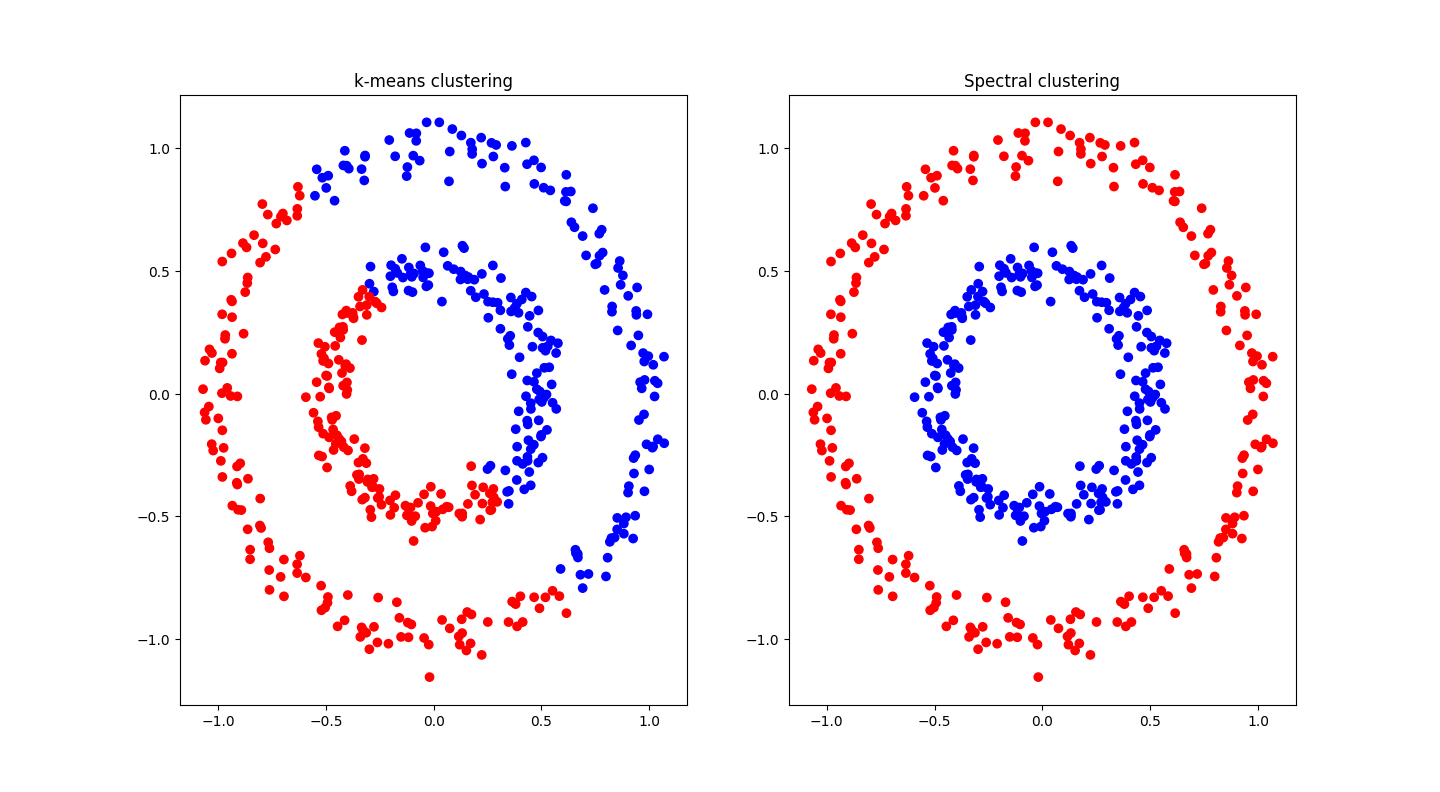
\includegraphics[width=0.7\linewidth]{figures/Fig1}
	\caption{Comparison between $k$-means clustering and spectral clustering on a toy dataset}
	\label{fig:fig1}
\end{figure}
However, due to it's relative recency and important practical applications, spectral clustering is still heavily studied today. It still has theoretical limitations that hinders it's performance. Improving the theory behind these algorithms is the goal of a team of researchers at LAAS-CNRS in Toulouse. This report presents the internship I have done in their team over the course of 6 weeks.\\
The goal of the internship was understanding classical spectral clustering (SC) in theory, then dive into \textbf{generalized spectral clustering} (GSC), the renewed theory of SC that the team is working on. I could then try helping the team by implementing SC and GSC on synthetic and real datasets, aiming to conduct experiments on the performance of these algorithms. This would hopefully lead to guiding theoretical research towards methods with the best experimental results, as good experimental results may be the sign of the existence of good theoretical results. \\
This internship allowed me to reinvest the mathematical tools learned during La Prépa in an Applied Mathematics context. To deeply understand the theory of SC and GSC, I also had to learn new mathematics, mostly in probability theory and functional analysis. I was also able to practice my Python programming skills and learn the art of presenting experimental results in a scientific way.
Most importantly, I was fully involved in the team, working at the lab and sharing everyday with it's researchers from all around the globe, discovering the world of academics.

\section{An overview of LAAS-CNRS}
LAAS-CNRS is a french research lab of the \textit{Centre National de la Recherche Scientifique} (CNRS), the biggest public research organism in France.
LAAS stands for \textit{Laboratoire d'analyse et d'architecture des systèmes} (Laboratory of system analysis and architecture). Behind this rather complex acronym lies 4 historical disciplinary fields : computer science, robotics, automatics and micro and nano systems.
The 'systems' considered in LAAS' research activites are of diffrent kinds :integrated systems, robotic systems, biological systems... \\
They fall in various application domains such as aeronautics and space, telecommunications, transports, production, services, security and defense, energy management, healthcare, environment and sustainable development.

\subsection{Foundation}
LAAS was created in 1968 under the name \textit{Laboratoire d'automatique et de ses applications spatiales} (Laboratory of automatics and it's spatial applications). Indeed, it is located in Toulouse, a leading city in spatial technology, near other important academic entities such as ENAC or CNES (National Centre for Space Studies).
\begin{figure}[H]
	\centering
	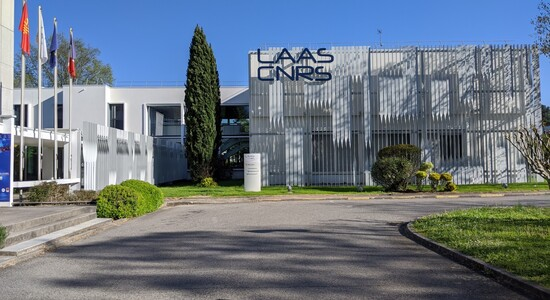
\includegraphics[width=0.4\linewidth]{figures/LAAS}
	\caption{LAAS-CNRS Facility in Toulouse}
	\label{fig:laas}
\end{figure}
\subsection{Lab organization and philosophy}
LAAS is the home of 6 research departments made up of 26 teams dedicated to their 4 disciplinary fields.
All departments combined, over 800 people work at LAAS, including 200 permanent researchers and 230 PhD students.
\begin{figure}[H]
	\centering
	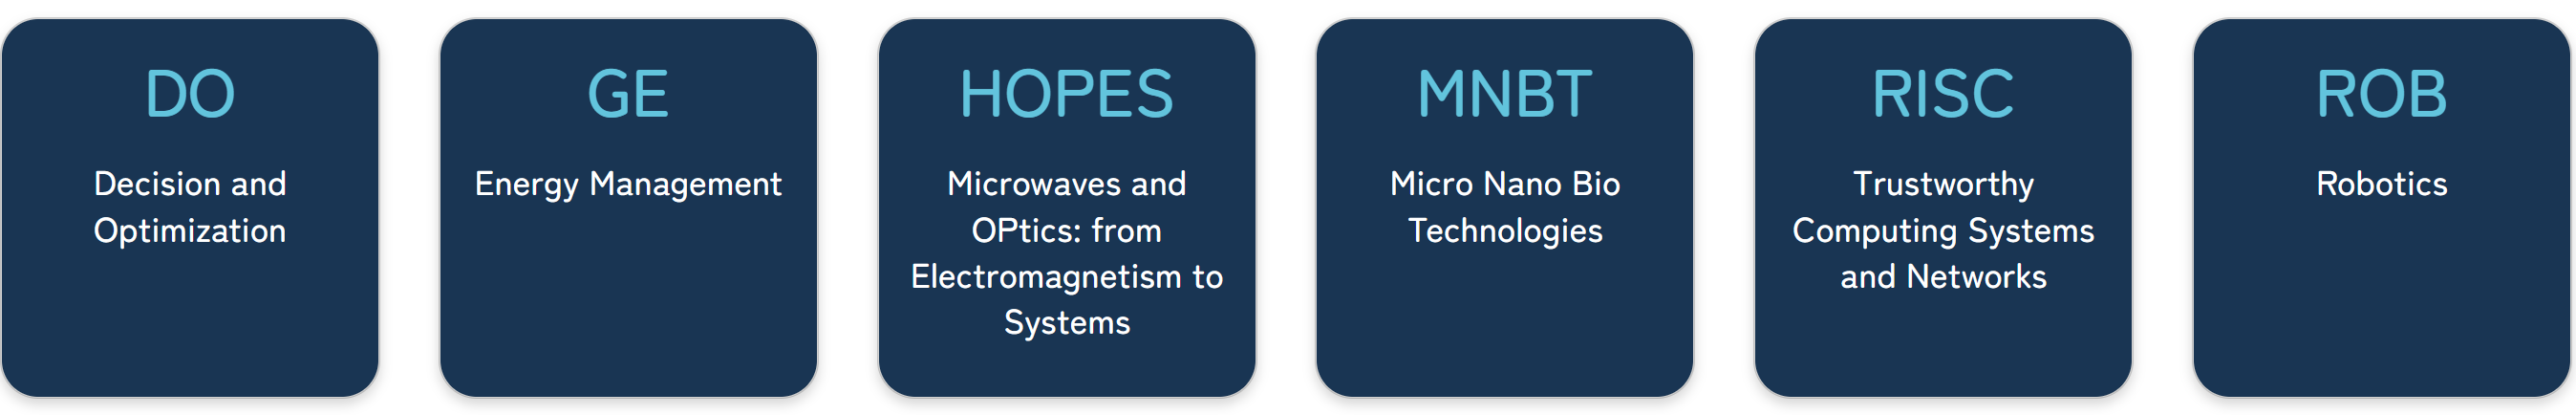
\includegraphics[width=0.6\linewidth]{figures/LAAS_Departments}
	\caption{LAAS' 6 research departments.}
	\label{fig:laasdepartments}
\end{figure}
The lab has a history of strong relationships with industry and works in a large number of collaborative projects with international, national and regional industries of all size. LAAS was one of the 20 first “Carnot Institutes” labeled in 2006, a label given to labs putting an emphasis on industry partnership.
LAAS also takes great advantage of it's pluridisciplinary nature : teams from different departments often collaborate to build projects. LAAS promotes transdisciplinary research through 4 strategic axes: Ambient intelligence, Living (biology, environment, medicine), Space and Energy. Examples include LAAS' mathematicians teaming up with robotics researchers to provide efficient Machine Learning (ML) algorithms for their projects.
\subsection{Daily life}
\end{document}